% Options for packages loaded elsewhere
\PassOptionsToPackage{unicode}{hyperref}
\PassOptionsToPackage{hyphens}{url}
%
\documentclass[
]{article}
\usepackage{amsmath,amssymb}
\usepackage{lmodern}
\usepackage{iftex}
\ifPDFTeX
  \usepackage[T1]{fontenc}
  \usepackage[utf8]{inputenc}
  \usepackage{textcomp} % provide euro and other symbols
\else % if luatex or xetex
  \usepackage{unicode-math}
  \defaultfontfeatures{Scale=MatchLowercase}
  \defaultfontfeatures[\rmfamily]{Ligatures=TeX,Scale=1}
\fi
% Use upquote if available, for straight quotes in verbatim environments
\IfFileExists{upquote.sty}{\usepackage{upquote}}{}
\IfFileExists{microtype.sty}{% use microtype if available
  \usepackage[]{microtype}
  \UseMicrotypeSet[protrusion]{basicmath} % disable protrusion for tt fonts
}{}
\makeatletter
\@ifundefined{KOMAClassName}{% if non-KOMA class
  \IfFileExists{parskip.sty}{%
    \usepackage{parskip}
  }{% else
    \setlength{\parindent}{0pt}
    \setlength{\parskip}{6pt plus 2pt minus 1pt}}
}{% if KOMA class
  \KOMAoptions{parskip=half}}
\makeatother
\usepackage{xcolor}
\usepackage[margin=1in]{geometry}
\usepackage{longtable,booktabs,array}
\usepackage{calc} % for calculating minipage widths
% Correct order of tables after \paragraph or \subparagraph
\usepackage{etoolbox}
\makeatletter
\patchcmd\longtable{\par}{\if@noskipsec\mbox{}\fi\par}{}{}
\makeatother
% Allow footnotes in longtable head/foot
\IfFileExists{footnotehyper.sty}{\usepackage{footnotehyper}}{\usepackage{footnote}}
\makesavenoteenv{longtable}
\usepackage{graphicx}
\makeatletter
\def\maxwidth{\ifdim\Gin@nat@width>\linewidth\linewidth\else\Gin@nat@width\fi}
\def\maxheight{\ifdim\Gin@nat@height>\textheight\textheight\else\Gin@nat@height\fi}
\makeatother
% Scale images if necessary, so that they will not overflow the page
% margins by default, and it is still possible to overwrite the defaults
% using explicit options in \includegraphics[width, height, ...]{}
\setkeys{Gin}{width=\maxwidth,height=\maxheight,keepaspectratio}
% Set default figure placement to htbp
\makeatletter
\def\fps@figure{htbp}
\makeatother
\setlength{\emergencystretch}{3em} % prevent overfull lines
\providecommand{\tightlist}{%
  \setlength{\itemsep}{0pt}\setlength{\parskip}{0pt}}
\setcounter{secnumdepth}{-\maxdimen} % remove section numbering
\usepackage{booktabs}
\usepackage{longtable}
\usepackage{array}
\usepackage{multirow}
\usepackage{wrapfig}
\usepackage{float}
\usepackage{colortbl}
\usepackage{pdflscape}
\usepackage{tabu}
\usepackage{threeparttable}
\usepackage{threeparttablex}
\usepackage[normalem]{ulem}
\usepackage{makecell}
\usepackage{xcolor}
\ifLuaTeX
  \usepackage{selnolig}  % disable illegal ligatures
\fi
\IfFileExists{bookmark.sty}{\usepackage{bookmark}}{\usepackage{hyperref}}
\IfFileExists{xurl.sty}{\usepackage{xurl}}{} % add URL line breaks if available
\urlstyle{same} % disable monospaced font for URLs
\hypersetup{
  hidelinks,
  pdfcreator={LaTeX via pandoc}}

\author{}
\date{\vspace{-2.5em}}

\begin{document}

\newpage

\hypertarget{ISCchumChapter}{%
\section{CASE STUDY 3: INSIDE SOUTH COAST CHUM -
NON-FRASER}\label{ISCchumChapter}}

\hypertarget{chum-context}{%
\subsection{CONTEXT}\label{chum-context}}

The Inside South Coast Chum - Non-Fraser SMU (abbreviated as ISC Chum)
includes seven CUs of Chum Salmon from rivers that drain into Johnstone
Strait and the Salish Sea along the mainland of British Columbia and the
east coast of Vancouver Island (Figure @ref(fig:chum-map);
@holtbyConservationUnitsPacific2007). This area includes deep fjords,
glaciers, large rivers, and small coastal streams. Chum salmon CUs
spawning in the Fraser River watershed are not included in this SMU.
They have been categorized as a separate `Inside South Coast Chum -
Fraser' SMU. While these two SMUs have substantial overlap in ocean
fisheries, they have been separated into two SMUs based on differences
in terminal fishery impacts and freshwater habitats.

\begin{figure}

{\centering 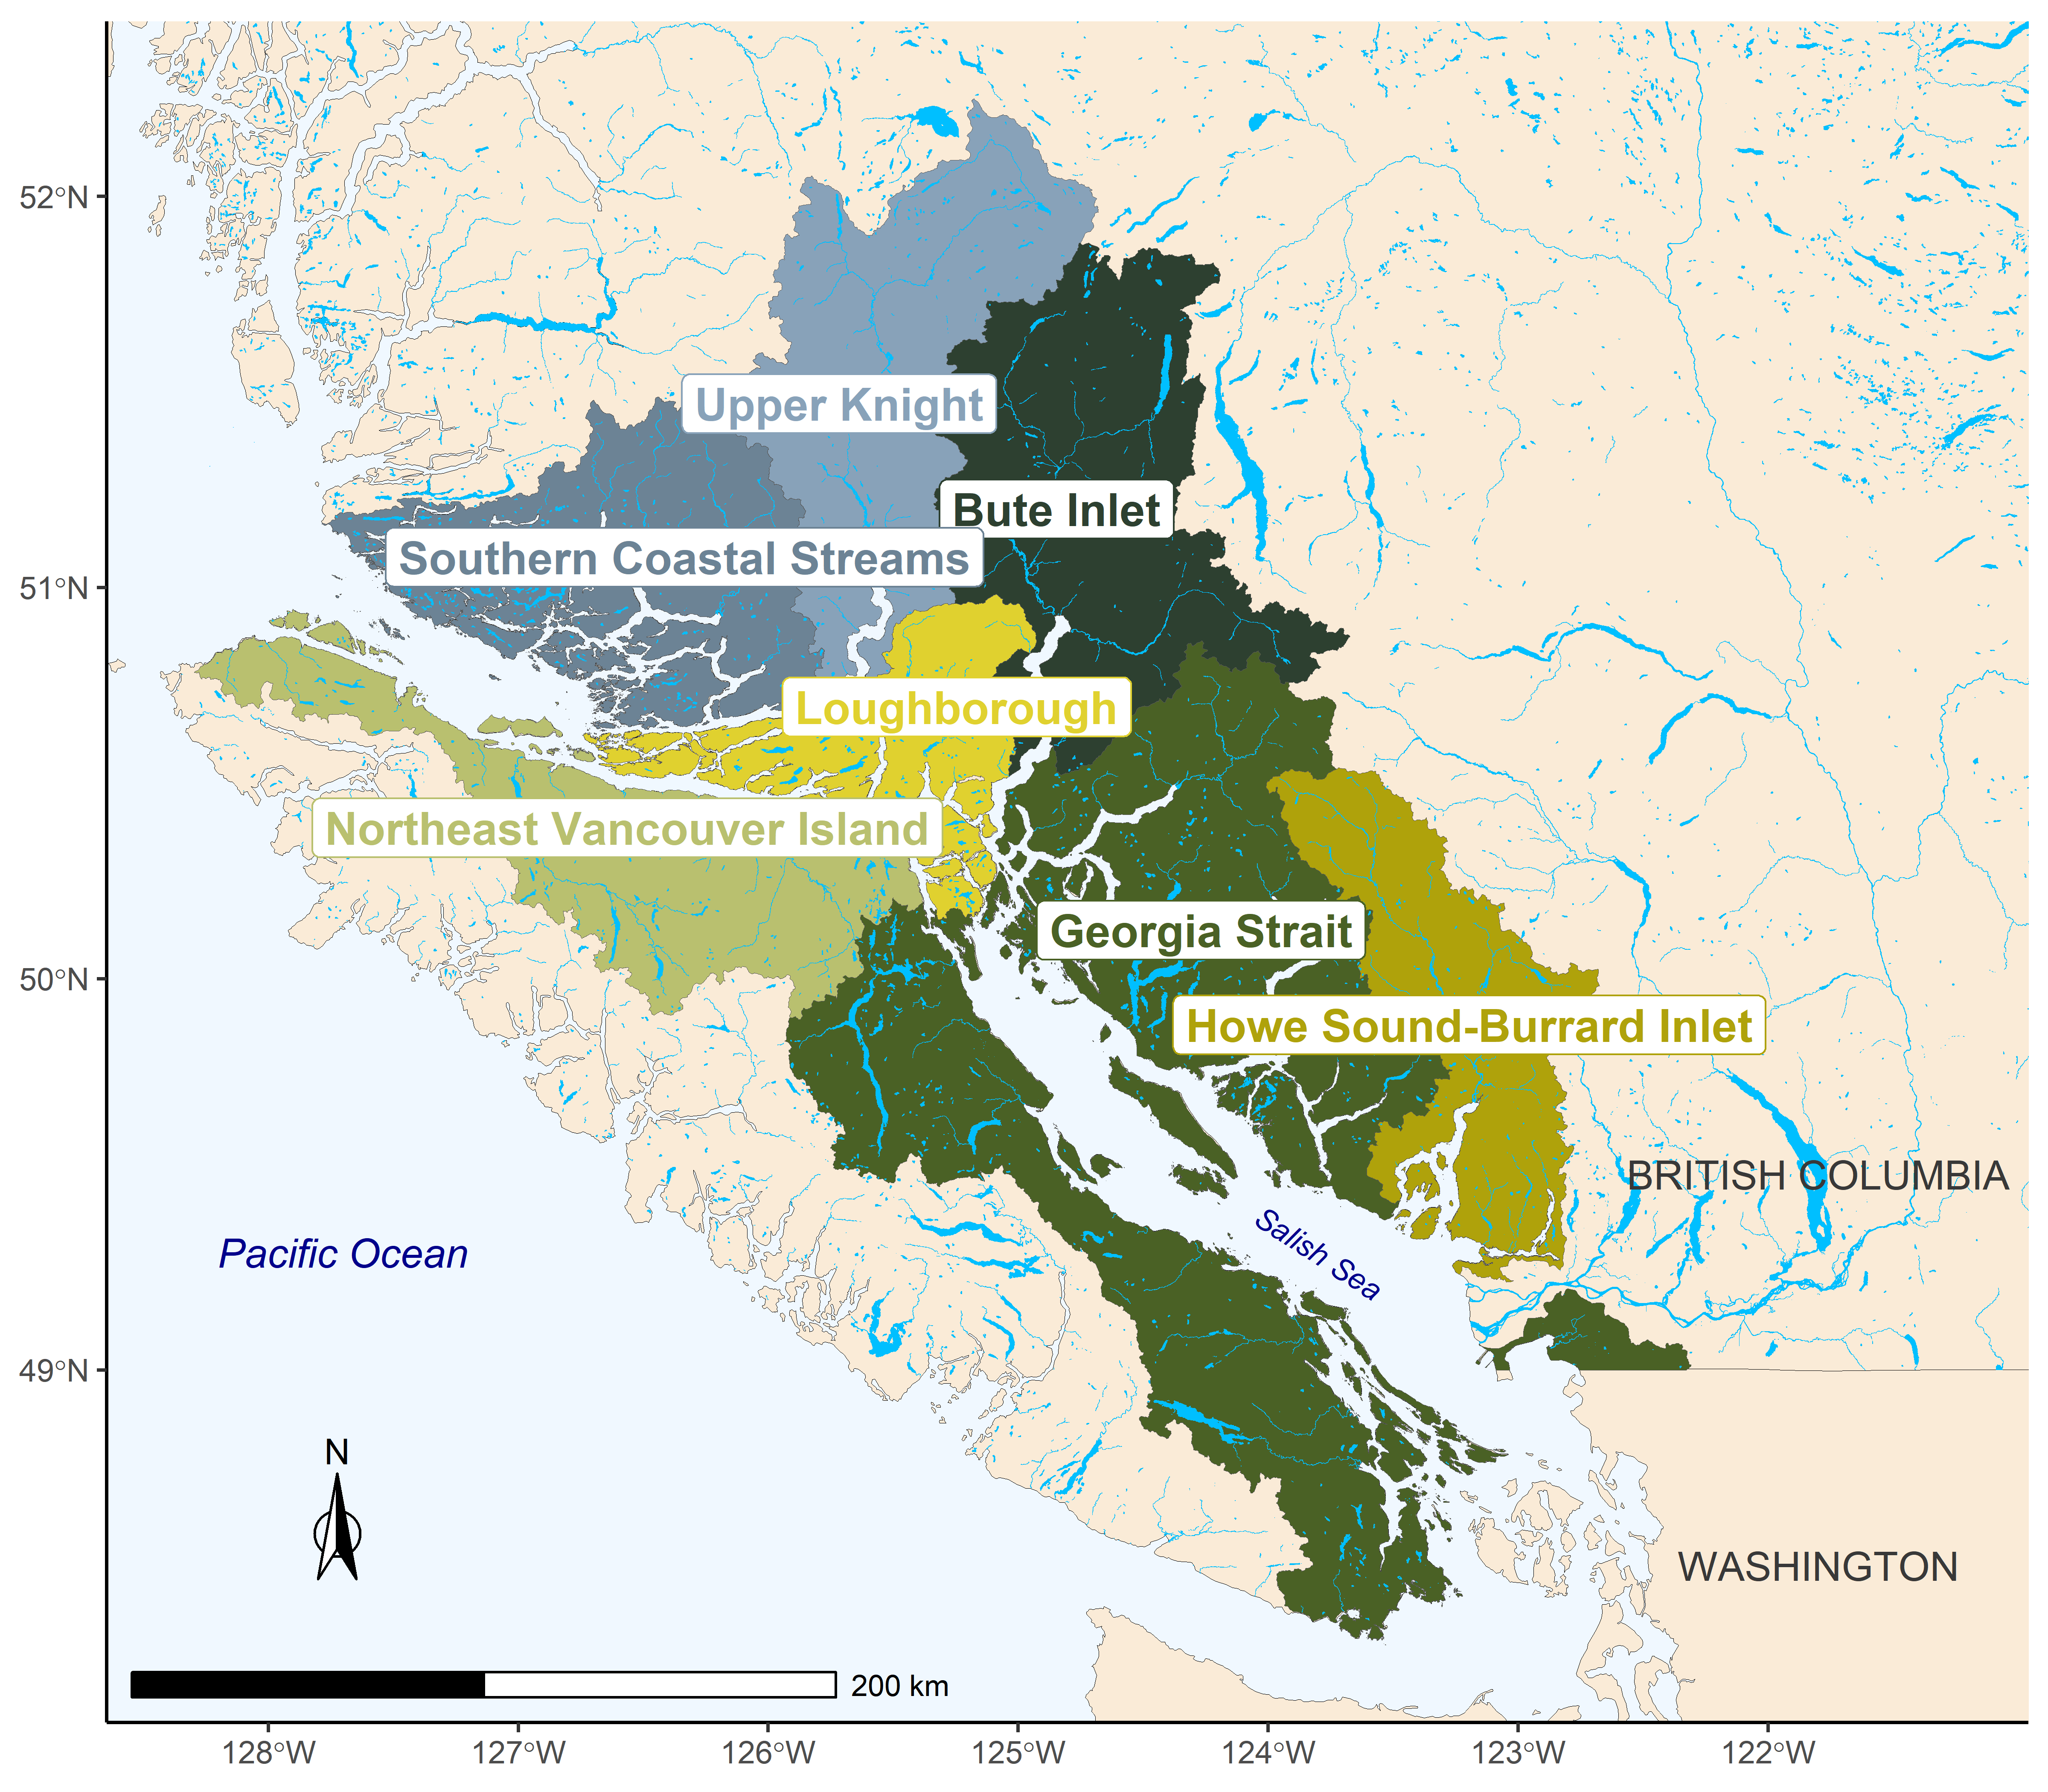
\includegraphics[width=66.67in]{figure/chum-map} 

}

\caption{The seven Conservation Units that make up the Inside South Coast Chum Stock Management Unit (not including Lower Fraser and Fraser Canyon Conservation Units).}\label{fig:chum-map}
\end{figure}
\linebreak

The ISC Chum SMU is considered data-limited. While escapement time
series are available for many streams starting in 1953, several series
are incomplete and require infilling assumptions (i.e., not all streams
counted each year, some CUs have no counts in some years). In addition,
run reconstructions of recruitment are uncertain, making the development
of benchmarks based on spawner and recruitment data problematic. There
are also no data on marine survival {[}although there are some
scale/growth data in @debertinMarineGrowthPatterns2017{]}. Other unique
characteristics of this SMU include high contrast in abundance among CUs
and relatively low correlation in abundance among CUs over time. The SMU
covers a large area with many diverse watersheds, flow regimes, and
ocean entry locations. Wild Salmon Policy status assessments have not
been done on any ISC Chum CUs. @godboutStockStatusWild2004 identified
long-term increases or variable abundance in Georgia Strait and Howe
Sound-Burrard Inlet and declines in Northeast Vancouver Island and
especially in the Southern Coastal Streams CU (from 1953-2002).
@holtEvaluatingBenchmarksBiological2018 found similar results in a
provisional assessment of status. At this time, a peer-reviewed WSP
status assessment has not been developed for ISC chum.

@holtGuidelinesDefiningLimitInpress provide steps for applying LRPs to
salmon SMUs, one of which is to identify if the status of data-deficient
CUs can be represented by other data-rich CUs. This is relevant for the
ISC Chum case study because two CUs have no observations in some years
(Upper Knight and Bute Inlet). To infer status of data-deficient CUs
from data-rich CUs, @holtGuidelinesDefiningLimitInpress recommend
providing evidence for similar threats, environmental drivers,
biological characteristics, and population capacity among CUs.

Upper Knight and Bute Inlet CUs are both associated with long fjords
that run from the Broughton Archipelago through the Coast Mountains.
They include rivers with headwaters in the Cariboo region farther inland
than other CUs in the SMU (Figure @ref(fig:chum-map)). Southern Coastal
Streams, Georgia Strait, and Howe Sound-Burrard Inlet also include
portions of the Coast Mountains and some glaciers, but to a lesser
extent and their inlets are shorter and their watersheds do not go as
far inland. Upper Knight and Bute Inlet are unique in that they are the
only CUs in the SMU that only include watersheds that drain into the
upper end of long inlets. They are both more remote than the other CUs,
which is partly why there are fewer observations over time for Chum with
fall run timing.

Chum from the Upper Knight and Bute Inlet CUs are exposed to different
threats to habitat, survival and productivity than the other five CUs in
both the freshwater and the early marine phase. While these two CUs
have, on average, lower impacts from forest harvest, impervious area,
and roads, they have larger impacts from forest defoliation and pests
{[}@pacificsalmonfoundationPacificSalmonExplorer2021{]}. They may also
have different levels of risk from disturbances such as glacier melt,
avalanches, debris flows, and floods because they have large melting
glaciers associated with lakes, steep slopes, and unstable terrain. In
the Bute Inlet CU, the glacial lake outburst flood that caused a debris
flow in the Southgate River in November 2020 is one example of such an
event. These events are capable of killing an entire brood year of
eggs/alevins and reshaping habitat with impacts on spawning habitat and
stream ecosystems for many years. They can also change water quality in
near shore marine habitats. These catastrophic events may be less likely
in watersheds with gentler topography and that lack glaciers and glacial
lakes.

Environmental drivers, biological characteristics, and population
capacity for Upper Knight and Bute Inlet CUs also differ from the other
five CUs. The hydrology of these two CUs likely differs from that of
other CUs with more low-lying topography. The two largest watersheds in
these CUs (Homathko and Klinaklini) fall within their own Freshwater
Adaptive Zone, which indicates unique freshwater habitat conditions
(Figure 76 and Table 52 in @holtbyConservationUnitsPacific2007). These
watersheds have large glaciers and high amounts of snowmelt, compared to
more low-elevation coastal watersheds with more rain-dominant
hydrographs. Marine conditions when smolts enter the ocean in these
systems may vary from that of the other five CUs, as they are entering
the upper ends of large fjords. Competition with other salmon in the
ocean and ocean conditions affect chum salmon in this SMU
{[}@debertinMarineGrowthPatterns2017;
@litzCompetitionOddyearPink2021{]}, although declines in Pink salmon
populations in this general area may suggest that these factors are not
affecting these CUs only. Regarding biological characteristics, Bute
Inlet and Upper Knight have a higher proportion of summer-run
populations of Chum (Table @ref(tab:CU-summary)). Recruits per spawner
of the Upper Knight and Bute Inlet CUs (estimated using CU-level
infilling, which introduces error) are more variable than for other CUs
in this SMU, exhibiting very productive years (\textgreater100 recruits
per spawner) and years with very low productivity. These CUs also have
lower habitat capacity, with fewer streams with fall timed Chum spawners
than the other CUs (Table @ref(tab:CU-summary)). Based on these
differences, we cannot infer the status for Bute Inlet and Upper Knight
from the other CUs. Note that these criteria used to evaluate whether
status can be inferred for these CUs extends to whether reliable spawner
escapement data can be infilled using escapement in the other CUs. Thus,
these CUs are dropped for years with no spawner data in this case study.

\needspace{0.35\textheight}

\begin{longtable}[]{@{}lcccc@{}}
\caption{The seven Conservation Units in the Inside South Coast Chum
Non-Fraser Stock Management Unit, and the number of streams in the fall
and summer runs. Note that only fall run streams were used in this study
due to run reconstruction methods. LBM = Lower Benchmark, UBM = Upper
Benchmark derived using the percentile method.}\tabularnewline
\toprule()
CU Name & Fall run streams & Summer run streams & LBM & UBM \\
\midrule()
\endfirsthead
\toprule()
CU Name & Fall run streams & Summer run streams & LBM & UBM \\
\midrule()
\endhead
Southern Coastal Streams & 23 & 8 & NA & NA \\
North East Vancouver Island & 17 & 0 & 50\% & 50\% \\
Upper Knight & 3 & 2 & 50\% & 50\% \\
Loughborough & 37 & 0 & 50\% & 50\% \\
Bute Inlet & 4 & 1 & NA & NA \\
Georgia Strait & 125 & 1 & 25\% & 50\% \\
Howe Sound-Burrard Inlet & 66 & 0 & 25\% & 50\% \\
\bottomrule()
\end{longtable}

\afterpage{\clearpage}

Previous evaluations of WSP benchmarks for Inner South Coast Chum have
shown that percentile benchmarks can be comparable to those based on
stock-recruit relationships when productivity is relatively high and
harvest is relatively low {[}@holtEvaluatingBenchmarksBiological2018{]}.
However, in some cases, percentile benchmarks may be inappropriate due
to low productivity or high harvest, resulting in a shifting baseline
{[}@holtEvaluatingBenchmarksBiological2018{]}.

We chose the ISC Chum SMU as a case study because we were interested in
exploring LRP options for a data-limited SMU without stock-recruitment
or habitat-based benchmarks. We applied LRPs based on two methods:
proportions of CUs above Red status, and aggregate abundance LRPs
estimated using the logistic regression approach.

\hypertarget{data}{%
\subsection{DATA}\label{data}}

We used the same data used in @holtEvaluatingBenchmarksBiological2018,
but updated with five additional years of data. Available data included
spawner abundance time series from 1959 - 2018 and corresponding
CU-level recruitment estimated from run reconstruction. Spawner
abundance series rely heavily on infilling; 60\% of observations (count
of spawners for an individual stream, in a given year) were missing and
needed to be infilled. We chose to apply infilling procedures for this
SMU when possible to develop metrics of wild spawner abundance since
infilling methods for this SMU have been previously peer reviewed
{[}@holtEvaluatingBenchmarksBiological2018{]}. This differs from the
approach taken for WCVI Chinook, in which infilling methods were not
implemented due to high and variable hatchery influences. Recruitment
data are considered highly uncertain for all ISC Chum CUs due to
uncertain assumptions required to assign mixed-fishery catch to CUs
within the run-reconstruction model. As a result, we did not consider
recruitment time-series to be reliable enough to estimate
stock-recruitment based benchmarks such as S\textsubscript{MSY} and
S\textsubscript{gen}. We did however use spawner recruit model fits to
provide approximate estimates of CU-level productivity, which are used
to inform the application of percentile-based benchmarks.

@vanwillInnerSouthCoast2014 provides more details on the data sources,
infilling procedures and run reconstruction, which were reproduced for
this study. We did not include the Lower Fraser or Fraser Canyon Chum
CUs. More details can be found in Appendix @ref(app:appendix-chum). We
removed three systems with extensive enhancement (Qualicum River and
Little Qualicum River from spawning channels, and Puntledge River from
hatchery production, all within the Georgia Strait CU). It is assumed
that the enhanced contribution to spawning was near 100\% for these
systems.

\hypertarget{cu-status-estimation}{%
\subsection{CU STATUS ESTIMATION}\label{cu-status-estimation}}

For this case study, we consider two approaches for characterizing CU
status: (1) Multidimensional algorithm within the Pacific Salmon Scanner
Tool, or Salmon Scanner (Pestal et al.~in prep.) and (2) CU-level
abundance relative to a percentile lower benchmark.

The first approach is a multidimensional approach consistent with
Canada's WSP, as recommended by @holtGuidelinesDefiningLimitInpress for
estimating CU status when using the CU status-based LRP approach. The
second approach is presented for comparison with the multidimensional
approach.

When applying the multidimensional algorithm used within the Salmon
Scanner to ISC Chum, we used percentile benchmarks when they were
available for a CU. For CUs in which percentile benchmarks were not
appropriate, the multidimensional algorithm used trends in spawner
abundance as a basis for assessing CU status (Figure
@ref(fig:decision-tree)). As a result, both of our approaches to CU
status estimation depend at least partially on percentile benchmarks.

Percentile benchmarks can be applied to assess status of CUs when other
data - like benchmarks based on productivity or habitat - are not
available or reliable {[}@holtEvaluatingBenchmarksBiological2018;
@clarkEvaluationPercentileApproach2014{]}. The suitability of percentile
benchmarks was evaluated for ISC Chum by
@holtEvaluatingBenchmarksBiological2018, who tested how well percentile
benchmarks matched benchmarks from stock-recruit parameters, using
retrospective and simulation analyses.
@holtEvaluatingBenchmarksBiological2018 also calculated benchmarks based
on stock-recruit model parameters for ISC Chum CUs, but did not
recommend them due to uncertainty in spawner and recruit data. They
tested how well a 25\% percentile benchmark (and higher values up to
50\%) compared to estimates of S\textsubscript{gen} for these CUs. They
found that percentile benchmarks (from 25-50\%) under moderate to high
harvest rates and low to moderate productivity tended to underestimate
`true' S\textsubscript{gen} values (estimated from the same data), which
would lead to optimistic and incorrect status assessments. More work on
alternatives to percentile benchmarks were needed in this case.

For this case study, percentile benchmarks were calculated using the raw
infilled time series of annual escapement (i.e., not smoothed). In
contrast, status for year \(i\) was determined by comparing the
generational mean (geometric mean on a 4-year window, ending with year
\(i\)) spawner abundance with the benchmark. This approach of using raw
(unsmoothed) escapements when calculating benchmarks, and generational
smoothed escapements when estimating CU status relative to benchmarks,
is consistent with the approaches taken for our other two case studies
for proortional LRPs.

\needspace{0.35\textheight}

\renewcommand*{\arraystretch}{1.5}
\begin{table}[ht]
\centering
\caption{Selected percentile-based lower and upper benchmarks identified to be similar or higher in value than stock-recruitment based benchmarks under the WSP, along gradients in productivity (Ricker $\alpha$) and average harvest rates. * denotes the low-productivity scenario where lower and upper Ricker-based benchmarks are very close to one another, resulting in lower and upper percentile-based benchmarks that are the same. Adapted from Table 6, Holt et al. 2018.}
\begin{tabular}{l l p{2.5cm} p{2.5cm} p{2.5cm}}
\hline       &     & \multicolumn{3}{l}{Harvest rate}\\ 
& & <20\% & 20-40\% & 40-60 \% \\
\hline
Productivity (Ricker $\alpha$) & >4 & 25th (lower)  50th (upper) & 25th (lower) 50th (upper) & 25th (lower) 50th (upper) \\
& 2.5-4 & 25th (lower) 50th (upper) & 25th (lower) 50th (upper) & Further evaluation required \\
& 1.5-2.5 & *50th (lower and upper) & Further evaluation required & Further evaluation required \\               
\hline
\end{tabular}
(\#tab:holt-tab6)
\end{table}

\afterpage{\clearpage}

Based on recommendations in @holtEvaluatingBenchmarksBiological2018
(Table @ref(tab:holt-tab6)), Georgia Strait and Howe Sound-Burrard Inlet
fall in the category of using 25\% as a lower benchmark and 50\% as an
upper benchmark (Ricker \(\alpha\) 2.5-4, harvest rate 20-40\%).
Loughborough, Northeast Vancouver Island, and Upper Knight (\(\alpha\)
1.5-2.5 and harvest rate 0-20\%) had a 50\% lower and upper benchmark
recommended. Bute Inlet (\(\alpha\) 1.5-2.5, harvest rate 20-40\%)
needed further evaluation and percentile benchmarks were not
recommended. Percentile benchmarks were also not recommended for
Southern Coastal Streams due to low productivity (\(\alpha\)
\textless1.5; Table @ref(tab:CU-summary)).

The methods for multidimensional assessments within the Salmon Scanner
are described in Section @ref(MethodsChapter). In applying the
multidimensional approach to ISC Chum, we used percentile benchmarks as
recommended in @holtEvaluatingBenchmarksBiological2018 for lower and
upper benchmarks for the five CUs that have appropriate percentiles
benchmarks identified (as described above). Percentile benchmarks were
not available for Bute Inlet and Southern Coastal Streams, in which case
the multidimensional algorithm used trends to assess CU status (Figure
@ref(fig:decision-tree)).

\hypertarget{lrp-estimation-cu-status-based}{%
\subsection{LRP ESTIMATION: CU STATUS
BASED}\label{lrp-estimation-cu-status-based}}

\hypertarget{methods}{%
\subsubsection{Methods}\label{methods}}

To derive CU status-based LRPs, we calculated the proportion of CUs that
had status estimates above the Red zone (or, above the lower percentile
benchmark). As with the Interior Fraser Coho and WCVI Chinook case
studies, we required all CUs to be above the Red zone for the ISC Chum
SMU to be classified as being above the LRP.

The single-metric approach to assessing CU status based on percentiles
has specific data requirements
{[}@holtEvaluatingBenchmarksBiological2018{]} while the multidimensional
approach can be applied to any CU with at least a consistent time-series
of spawner abundances. To compare LRPs based on CU assessment from these
two approaches we compared data subsets including those that used the
same data for each method, and all appropriate data for each method. We
evaluated six different combinations of data and LRP methods (Table
@ref(tab:LRP-scenarios)). \needspace{0.35\textheight}

\renewcommand*{\arraystretch}{1.5}
\begin{table}[ht]
\centering
\caption{Scenarios using different subsets of data (CU names abbreviated) and methods to assign LRP status. 'Y' indicates a full time series, 'YP' indicates a time series was included but is partial (missing years that required CU-level infilling which wer omitted). Bute Inlet and Southern Coastal Streams do not have appropriate percentile benchmarks. 'Full' scenarios use only years with full time series (no CU-level infilled CUs) and 'partial' scenarios include CU-level infilled CUs but drop years with CU-level infilling for those CUs.}
\begin{tabular}{l c c c c c c c }
\hline    
Scenario Name &   \rotatebox{90}{Southern Coastal Streams} &   \rotatebox{90}{ North East Vancouver Island} &  \rotatebox{90}{ Upper Knight} &  \rotatebox{90}{ Loughborough} &  \rotatebox{90}{ Bute Inlet} & \rotatebox{90}{ Georgia Strait} & \rotatebox{90}{ Howe Sound-Burrard Inlet}\\ 
\hline
1. CUbased: Scanner: 4CUs full       & - & Y & -  & Y & -  & Y & Y \\
2. CUbased: Percentile: 4CUs full    & - & Y & -  & Y & -  & Y & Y \\
3. CUbased: Scanner: 5CUs partial    & - & Y & YP & Y & -  & Y & Y \\
4. CUbased: Percentile: 5CUs partial & - & Y & YP & Y & -  & Y & Y \\
5. CUbased: Scanner: 5CUs full       & Y & Y & -  & Y & -  & Y & Y \\
6. CUbased: Scanner: 7CUs partial    & Y & Y & YP & Y & YP & Y & Y \\
\hline
\end{tabular}
(\#tab:LRP-scenarios)
\end{table}

\afterpage{\clearpage}

When describing ISC Chum LRP scenarios in Table @ref(tab:LRP-scenarios)
and throughout this case study, we use the following labeling
convention: \emph{Metric : CU Status Method : Data Scenario}. `Metric'
refers to the choice to base all ISC Chum LRPs on the proportion of CUs
above Red CU status (CUbased). The `CU Status Method' can be based on
the multidimensional algorithm within the Salmon Scanner (Scanner) or on
a single percentile benchmark used to characterize CU status
(Percentile). Finally, `Data Scenario' labels indicate both the number
of CUs represented (4, 5, or 7) and the completeness of the time series
(Full or Partial). `Full' scenarios only included CUs with complete time
series (no CUs with missing years). `Partial' scenarios included CUs
with incomplete time series (years that did not have observations in
those CUs were omitted). When using percentile benchmarks in these
scenarios, we used percentiles based on
@holtEvaluatingBenchmarksBiological2018. The benchmarks were estimated
using the entire time series.

For Scenarios 2 and 4 in Table @ref(tab:LRP-scenarios), we used CU
status based on percentile benchmarks that are determined by
productivity and historical exploitation, as outlined in
@holtEvaluatingBenchmarksBiological2018. This method used annual
escapement values to calculate benchmarks and the generational mean of
escapement (geometric mean over 4 years) to assess status in each year.
Scenario 2 includes the four CUs that had complete time series
(observations in each year, no CU-level infilling) and that also had
appropriate percentile benchmarks (Table @ref(tab:LRP-scenarios)). For
example, Upper Knight was excluded because it did not have a complete
time series, Southern Coastal Streams was excluded because it does not
have an appropriate percentile benchmark, and Bute Inlet was excluded
for both of these reasons. We then relaxed this requirement for all CUs
to have data in all years and included all CUs that meet the constraints
of @holtEvaluatingBenchmarksBiological2018 even if they had missing data
for some years (Scenario 4). This scenario included Upper Knight in some
years, which meant that it had five CUs in some years and four in
others. Thus, the power to detect Red status varied among years in
Scenario 4, using more of the available data than Scenario 2.

For Scenarios 1, 3, 5 and 6 in Table @ref(tab:LRP-scenarios), we used
status based on the multidimensional algorithm within the Salmon
Scanner. To compare results between status on a single metric (abundance
relative to percentile benchmarks) and the multidimensional approach, we
applied the multidimensional algorithm to the same two data sets used
for percentiles, i.e., using same CUs and years. For examples, Scenarios
1 and 2 use the same data, and Scenarios 3 and 4 use the same data.
Because the multidimensional assessments do not require abundance-based
benchmarks to assign status, this method could also be used for CUs that
did not have appropriate percentile benchmarks (Southern Coastal Streams
and Bute Inlet). Scenario 5 only included CUs with a full time series,
and Scenario 6 included Upper Knight and Bute Inlet, which had some
missing years.

\hypertarget{results}{%
\subsubsection{Results}\label{results}}

\textbf{CU Status Based on the Multidimensional Approach within the
Salmon Scanner}

Using the CU status based on the multidimensional approach within the
Salmon Scanner, two out of five CUs with data in the most recent year of
data (2018) would be above their lower benchmark (Amber or Green zone)
and three would be below (Red zone; Figure
@ref(fig:chum-CU-status-tree)). Over the time series, status for Howe
Sound-Burrard Inlet and Georgia Strait has improved, while status in
other CUs has declined or switched from Green to Red several times.

\begin{figure}

{\centering 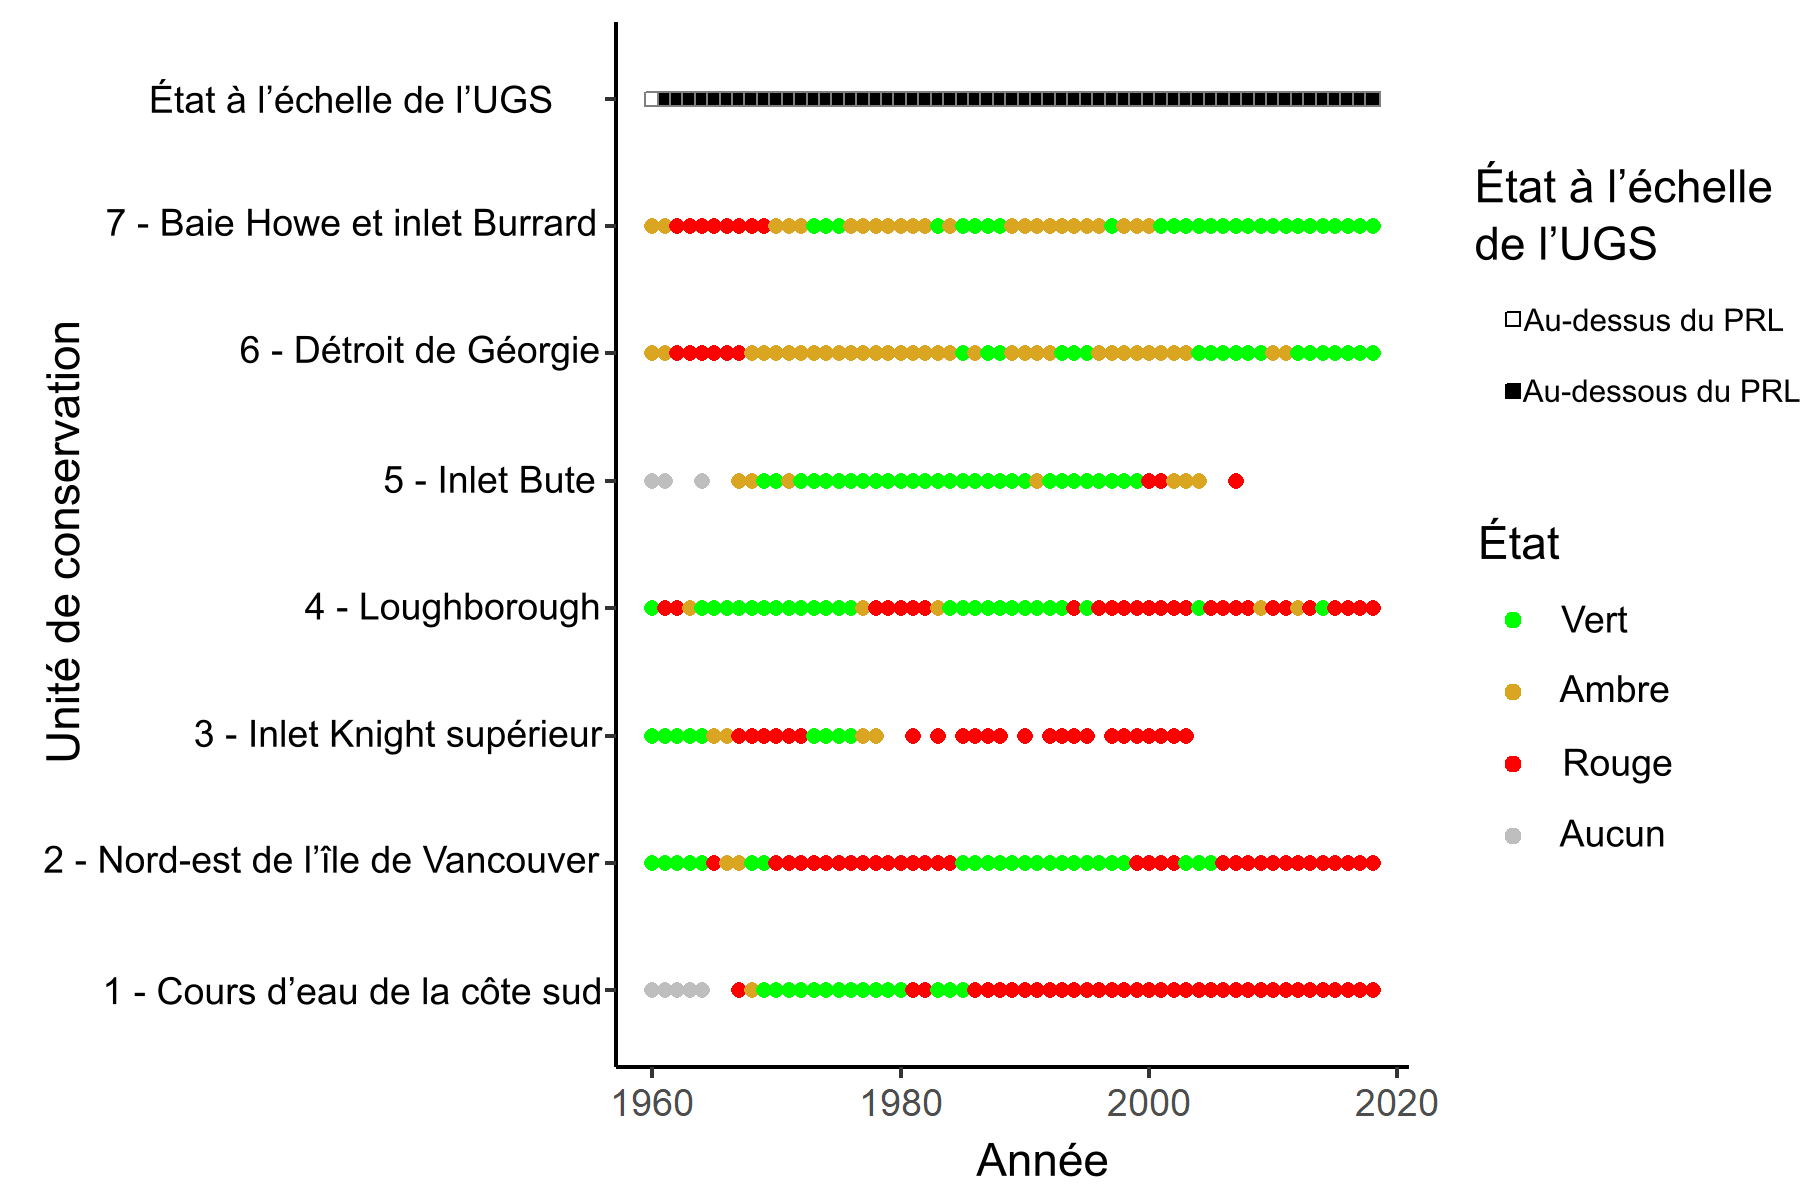
\includegraphics[width=25in]{figure/fig_status_by_CU_perc_RelAbd} 

}

\caption{Status of CUs based on multi-dimensional Salmon Scanner. Years with CU-level infilling were not included. The top row shows the overall SMU status based on the CU status-based LRP of all CUs being above Red status.}\label{fig:chum-CU-status-tree}
\end{figure}

\hfill\break
~

\textbf{CU Status Based on Percentile Benchmarks}

Two out of four CUs were below their percentile lower benchmark in 2018
(Figure @ref(fig:chum-perc-status-static)). Howe Sound-Burrard Inlet and
Georgia Strait had status above their lower benchmarks, and Upper Knight
did not have observations in 2018. Status for North East Vancouver
Island and Loughborough was occasionally above the Red zone before the
2000s, but has been mainly Red for the past \(\sim\) 20 years. Georgia
Strait and Howe Sound-Burrard Inlet have been above Red status in every
since \(\sim\) 1970. Upper Knight has been mainly Red status except for
two short periods in in the 1960s and 1970s, and did not have any
observations since 2004.

\begin{figure}

{\centering 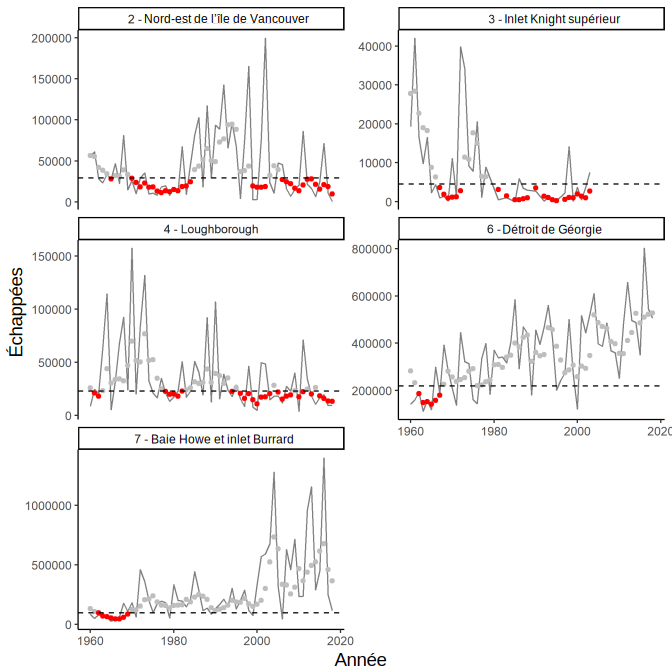
\includegraphics[width=29.17in]{figure/fig_percentile_bm_rel_abd} 

}

\caption{Spawner escapement (solid black line) with generational mean (4-year rolling geometric mean) of escapement in points. Dashed lines indicate percentile lower benchmarks. Red points indicate years when the generational mean of abundance was below the lower benchmark, and gray points indicate when it was above. Southern Coastal Streams and Bute Inlet are omitted because they do not have appropriate percentile benchmarks due to low productivity and moderate to high harvest. Note that Upper Knight is missing observations in 1979-1980, 1982, 1984, 1989, 1991, 1996, and 2004-2018.}\label{fig:chum-perc-status-static}
\end{figure}

In supplementary analyses, we evaluated percentile benchmarks
retrospectively for each year in the time series using only data prior
to that year. As more years of data were included, percentile benchmarks
increased over time for Georgia Strait (especially the
50\textsuperscript{th} percentile) and had modest increases for Howe
Sound-Burrard Inlet (Figure @ref(fig:chum-perc-retro)). Percentile
benchmarks decreased by a small amount for Loughborough and North East
Vancouver Island. Southern Coastal Stream shows evidence of shifting
baselines, as the percentiles decrease over time following a general
decline in abundances (Figure @ref(fig:chum-perc-retro)). Upper Knight
also shows this pattern but to a lesser extent.

\hypertarget{lrp-estimation-aggregate-abundance-logistic-regression-lrps}{%
\subsection{LRP ESTIMATION: AGGREGATE ABUNDANCE LOGISTIC REGRESSION
LRPS}\label{lrp-estimation-aggregate-abundance-logistic-regression-lrps}}

\hypertarget{methods-1}{%
\subsubsection{Methods}\label{methods-1}}

We evaluated whether the proportion of CUs above their lower benchmark
could be predicted by aggregate abundance using logistic regression
models. We tested this using percentile benchmarks. While we initially
considered logistic regression LRPs that used S\textsubscript{gen} as a
lower CU benchmark instead of percentiles, we decided to drop this
approach due to unreliable stock-recruit data. Using recruitment data
would not satisfy reliability principles in
@holtGuidelinesDefiningLimitInpress. These methods used four CUs with
over 50 years of data and appropriate percentile benchmarks (North East
Vancouver Island, Loughborough, Georgia Strait, and Howe Sound-Burrard
Inlet). Aggregate abundance (predictor variable) was calculated using
only these four CUs. We omitted Bute Inlet and Upper Knight (both had
CU-level infilling in recent years) and Southern Coastal Streams (no
appropriate percentile benchmark). Refer to Section @ref(MethodsChapter)
for more details.

Due to poor logistic model fits using the entire 1953-2018 time series,
we did not conduct retrospective analyses of logistic regression LRPs
for this SMU as was done for the Interior Fraser River Coho case study.
The characteristics of the data that led to poor logistic model fits are
highlighted in the results section below.

Projection LRPs are an alternative aggregate abundance LRP that we did
not consider for this SMU due to lack of reliable stock-recruitment
parameter estimates for component CUs. However, this approach could be
considered in future analyses given consensus on model structure and
parameterization that provide realistic uncertainties in projections of
population dynamics.

\hypertarget{results-1}{%
\subsubsection{Results}\label{results-1}}

The logistic model predicting whether all CUs were above their benchmark
based on aggregate abundance fit the data poorly (Figure
@ref(fig:chum-logistic-perc)). The sum of abundance for all CUs in a
given year was not a good predictor of whether those CUs were above
their benchmarks in that year. Years with high aggregate abundance but
with some CUs below their benchmark make a logistic model unsuitable for
the purpose of estimating which aggregate abundance is linked to a high
probability of each component CU being above its lower benchmark.

The diagnostics for the logistic regression indicated that the model fit
was poor (Table @ref(tab:logistic-diag-chum), Figure
@ref(fig:chum-logistic-perc)). Pseudo \(R^2\) was low (0.03), indicating
a poor fit. The Box-Tidwell test indicated a significant lack of
linearity in the relationship between aggregate abundance and log-odds
(p-value = 0.02), which means that the assumption that the relationship
between aggregate abundance and log-odds is linear was not met.
Including aggregate abundance in the model did not improve fit over the
null model based on a Goodness of fit p-value of 0.13
(\textgreater0.05). The ratio of correct classifications (above below
LRP) relative to all classification was 0.7 based an LRP at p=0.5. Note
that this method tends to have overly optimistic values when the data
used to fit the logistic model and to evaluate classification accuracy
are the same. The Wald p-value was not significant for \(B_{1}\)
(p=0.19, the coefficient for aggregate abundances). There was no
evidence of outliers or autocorrelation in residual deviations. Despite
meeting the last two assumptions (no autocorrelation or outliers), they
were not enough to overcome the deficiencies identified by the other
diagnostic criteria. Therefore, logistic regression LRPs are not
presented here.

\begin{figure}

{\centering \includegraphics{figure/chum-logistic-perc} 

}

\caption{Logistic regression of whether escapement of all component CUs were above their percentile benchmarks based on aggregate abundance, for Inside South Coast Chum SMU. Includes CUs where percentile benchmarks were appropriate (no Bute Inlet, Upper Knight, or Southern Coastal Streams)}\label{fig:chum-logistic-perc}
\end{figure}

\needspace{0.35\textheight}

\begin{longtable}[]{@{}
  >{\raggedright\arraybackslash}p{(\columnwidth - 2\tabcolsep) * \real{0.3611}}
  >{\raggedright\arraybackslash}p{(\columnwidth - 2\tabcolsep) * \real{0.2083}}@{}}
\caption{(\#tab:logistic-diag-chum) Model diagnostic statistics from
logistic regression LRP using percentile benchmarks. A description of
diagnostic tests is provided in Section 2. Hit ratios are shown for
p=0.5.}\tabularnewline
\toprule()
\begin{minipage}[b]{\linewidth}\raggedright
Diagnostic Test
\end{minipage} & \begin{minipage}[b]{\linewidth}\raggedright
Value
\end{minipage} \\
\midrule()
\endfirsthead
\toprule()
\begin{minipage}[b]{\linewidth}\raggedright
Diagnostic Test
\end{minipage} & \begin{minipage}[b]{\linewidth}\raggedright
Value
\end{minipage} \\
\midrule()
\endhead
Box-Tidwell p-value & 0.02 \\
Max. deviance residual & 1.69 \\
AR-1 & 0.14 \\
Wald p-value & 0.19 \\
Goodness-of-fit p-value & 0.13 \\
Pseudo-\(R^2\) & 0.03 \\
Hit Ratio (p= 50\%) & 0.7 \\
\bottomrule()
\end{longtable}

\afterpage{\clearpage}

Several factors led to these poor model fits. The Inside South Coast
Chum SMU is made up of seven CUs that vary in their escapement
abundance. In many years, escapement in Georgia Strait and Howe
Sound-Burrard Inlet is greater than in other CUs by two orders of
magnitude (Figure @ref(fig:chum-spawner-distribution)). In addition, the
correlation in escapement among these seven CUs is low (Figure
@ref(fig:chum-spawner-corr)). These characteristics mean that the
aggregate abundance may be high due to one or more CUs with high
escapements, while one more smaller CUs are below their benchmark. High
aggregate escapements do not mean that all CUs are above their
benchmark. The low pairwise correlations in CU escapements are likely
due to the SMU covering a large area, with varying numbers of
populations affected by both local and regional factors, as described in
Sectoin @ref(chum-context).

\begin{figure}

{\centering 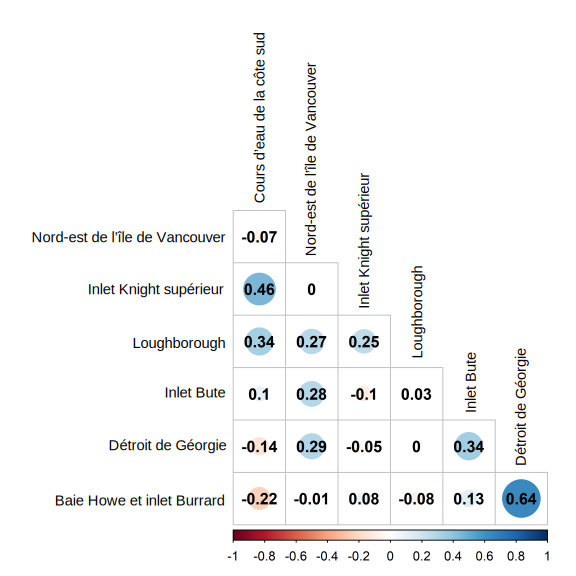
\includegraphics[width=0.8\linewidth]{figure/chum-spawners-corr} 

}

\caption{Pairwise correlations of spawner abundance between Inside South Coast Chum Conservation Units.}\label{fig:chum-spawner-corr}
\end{figure}
\linebreak

In a preliminary retrospective analysis, the logistic model fits were
more appropriate using a truncated portion of the data that ended in the
1980s. Although logistic regression may be used to estimated LRPs based
on aggregate abundance in SMUs where abundance is more even among CUs
and escapements are more correlated, these relationships may not remain
static and could break down over time.

\hypertarget{historical-evaluation-of-status-across-lrp-methods}{%
\subsection{HISTORICAL EVALUATION OF STATUS ACROSS LRP
METHODS}\label{historical-evaluation-of-status-across-lrp-methods}}

The ISC Chum SMU was consistently below the LRP for large portions of
the historical time series, regardless of LRP estimation method (Figure
@ref(fig:chum-LRP-compare)). While the aggregate abundance of the SMU
increased over time, SMU status remained below the LRP in every year of
the past two decades except 2004 for all estimation methods. These
results were mainly due to the tendency of Georgia Strait and Burrard
Inlet-Howe Sound CUs to have high and increasing abundances while
smaller CUs, such as North East Vancouver Island, Loughborough, and
Southern Coastal Streams, remained low (Figures
@ref(fig:chum-perc-status-static), @ref(fig:chum-escapement-infill)).

\begin{figure}

{\centering 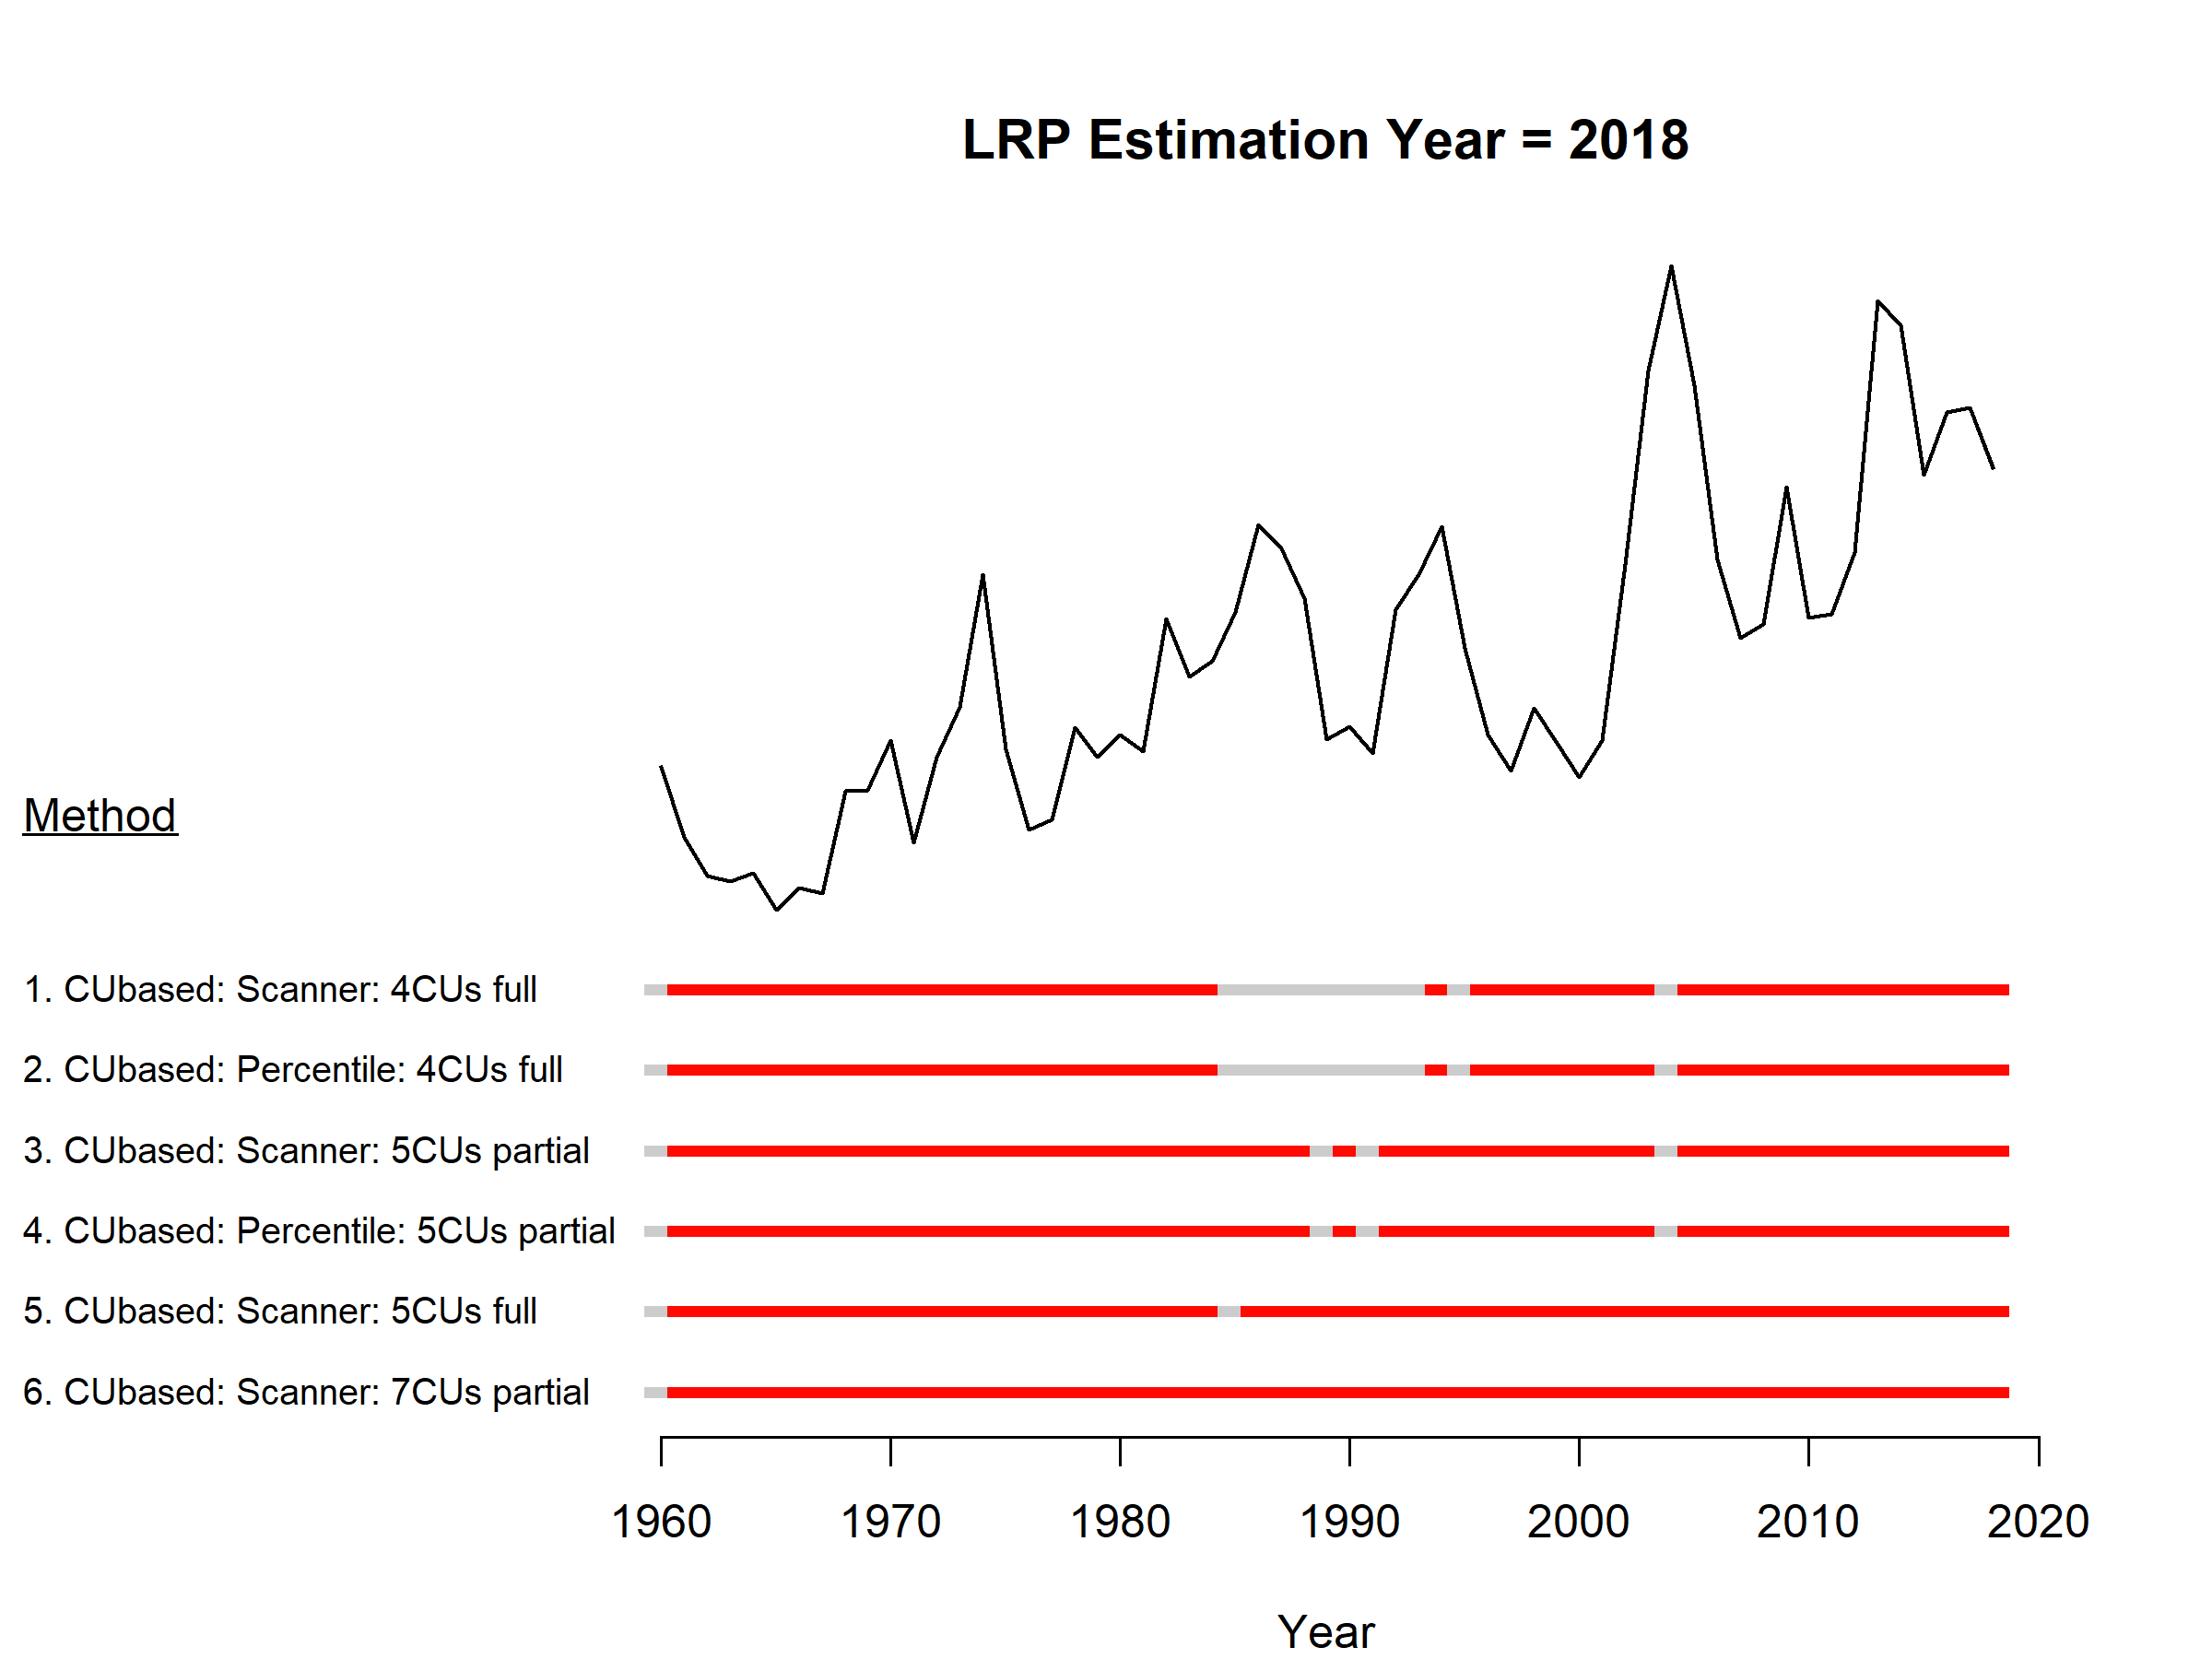
\includegraphics[width=33.33in]{figure/chum-compare-LRP-methods} 

}

\caption{Comparison of LRP status (red = below LRP, gray = above LRP) for six scenarios. The black line shows aggregate abundance. Scenarios 1-3 and 6 do not include Bute Inlet or Southern Coastal Streams (no appropriate percentile benchmarks). 'Full' scenarios use only years with full time series (no CU-level infilled CUs) and 'partial' scenarios include CU-level infilled CUs but drop years with CU-level infilling for those CUs.}\label{fig:chum-LRP-compare}
\end{figure}
\linebreak

When using the same data, LRP status based on a single metric on
abundances relative to percentile benchmarks and the multidimensional
approach within the Salmon Scanner were identical (Figure
@ref(fig:chum-LRP-compare)). This result can be seen by comparing
Scenario 1 and 2 and Scenario 3 and 4. These identical results occur
because all CUs in Scenarios 1-4 have percentile benchmarks and never
drop below 1500 fish, which means that the multidimensional approach
relies on percentile benchmarks to assess CU status for all CUs in all
years. If some CUs did not have percentile benchmarks, requiring trends
to be used instead, or if their absolute abundances dropped below 1500
spawners, then the two approaches could have led to different results.

In this case study, adding more data changed the number of years that
the SMU was below the LRP. Scenario 6 (most data) had the most years
below the LRP, with every year after the first being below the LRP
(Figure @ref(fig:chum-LRP-compare), Table @ref(tab:LRP-scenarios)). A
comparison of Scenarios 2 and 4, which are both based on percentile
benchmarks, shows that including more data (Scenario 4) results in more
years below the LRP. A comparison of Scenarios 5 and 6 (Salmon Scanner),
shows that including more observations results in one year switching
from above the LRP to below it, with the addition of data from two CUs
with partial time series. Finally, a comparison of Scenarios 4 and 6
(where Scenario 6 had two more CUs than Scenario 4), shows that three
years switched from above the LRP to below, as the two CUs without
percentile benchmarks are added.

We found that SMU status can be below the LRP even if the aggregate
abundance increases (Figure @ref(fig:chum-LRP-compare)). For ISC Chum,
this is mainly due to years with high abundances of Georgia Strait and
Howe Sound-Burrard Inlet and low abundances and Red status in other,
smaller CUs, such as Southern Coastal Streams. The moderate correlation
in spawner abundances in Georgia Strait and Howe Sound-Burrard Inlet
exacerbates this pattern (Figure @ref(fig:chum-spawner-corr)). This
highlights the importance of including metrics of status at the CU
level, which influence the overall SMU status.

\hypertarget{discussion}{%
\subsection{DISCUSSION}\label{discussion}}

As a data-limited SMU, the ISC Chum case study had unique
characteristics to inform the guidelines for LRP development. We found
that only the CU status-based LRP were applicable to this SMU, which is
based on individual CU status. Because there were no reliable
stock-recruit parameter estimates, we relied on data-limited methods to
estimate CU status. We assessed CU status based on abundance relative to
percentile benchmarks alone, or on a combination of percentiles and
trends using the multidimensional algorithm within the Salmon Scanner.
The use of the multidimensional algorithm was particularly valuable
because percentile benchmarks were not appropriate for two of the CUs
(Bute Inlet and Southern Coastal Streams, Table @ref(tab:CU-summary)).
Missing data also required decisions to be made about which CUs to
include in which years. We used this case study to explore how sensitive
CU status-based LRPs were to the decisions on number of CUs, and years
of data to include in the analysis.

Using a multidimensional approach allowed us to include two CUs that did
not have appropriate percentile benchmarks (Bute Inlet and Southern
Coastal Streams). It allowed all seven CUs to be included when assessing
SMU status by allowing alternative trend-based metrics to be considered.
The seven-CU partial case provided the most pessimistic status of the
scenarios considered as this approach used the most data. It resulted
with the most years of the SMU being below the LRP (Figure
@ref(fig:chum-LRP-compare)). This multidimensional approach is
especially useful for SMUs with a mix of data qualities and benchmark
types, including those with and without relative abundance benchmarks.
Like any approach to assess LRPs, the underlying data, and benchmarks
applied (if abundance benchmarks can be used) should be verified by
experts. In its current form, the multidimensional algorithm within th
Salmon Scanner relies on whether abundance is \(<\) 0.79\(\times\) the
long-term geometric average and whether abundances are \(>\) 1500 in the
absence of abundance-based benchmarks. It is worth noting that this
long-term geometric average may also be sensitive to shifting baselines.
This is another reason for experts to thoroughly review the data before
any status assessment is made.

This case study highlighted requirements and limitations of percentile
benchmarks on data-limited CUs. Shifting baselines are one of the
challenges of applying this method. If abundance has decreased over
time, the resulting percentile benchmark will also decrease as more data
is included (Figure @ref(fig:chum-perc-retro)). This can arise from a
decrease in abundance in the period of data or by an unrecorded high
level of abundance before the period of data followed by a decrease
before data are available. Thus, a CU with low abundance could be Green
status based on the current benchmark, but would be Red using a
benchmark with data before decreases in abundance. The result is an
overly optimistic view of current status that does not reflect the
reality of long-term declines. Two CUs (Southern Coastal Streams and
Upper Knight) showed evidence of shifting baselines as abundances
decreased over the last several decades (Figure
@ref(fig:chum-perc-retro)). Decreasing productivity can exacerbate this
pattern. As productivity decreases, a larger abundance of spawners would
be required to produce the same number of recruits. Experts should
thoroughly review historical abundance data and determine where shifting
baselines may be occurring, and can adjust benchmarks accordingly. In
some cases it may be appropriate to choose benchmarks based on
historical data or information prior to declines to avoid shifting
baselines {[}@holtCautionsUsingPercentilebased2015{]}. Thus, while they
are useful for CUs that lack reliable stock-recruit information, they
cannot be used universally on data-limited CUs.

Existing guidelines and cautions should be incorporated into any LRP
analysis using percentile benchmarks. We followed guidelines from
@holtEvaluatingBenchmarksBiological2018 and did not use percentile
benchmarks for CUs with low productivity and high exploitation rate
(Tables @ref(tab:CU-summary), @ref(tab:holt-tab6)). In their simulation
study, percentile-based benchmarks overestimated status with harvest
rates \textgreater40\% and \(\alpha\) \textless4, or harvest rates
20-40\% and \(\alpha\) \textless2.5. In these cases of low productivity
and high harvest rates, more exploration could be done on alternative
benchmarks. These could include benchmarks based on Traditional
Ecological Knowledge, habitat availability, or other information. If
productivity and/or harvest is unknown, low contrast in escapement
time-series could be indicators of cases where percentile benchmarks may
not be appropriate {[}@holtEvaluatingBenchmarksBiological2018{]}. We
also note that cases with identical lower and upper benchmarks carry the
risk of moving immediately from Green to Red status with time in the
Amber status zone (North East Vancouver Island, Upper Knight,
Loughborough, Table @ref(tab:CU-summary)). CUs with shorter time series
also have the risk of unreliable percentile benchmarks. Confidence
intervals for percentile benchmarks can also be derived by bootstrapping
escapement data, accounting for autocorrelation in time-series
{[}@peacockEvaluatingConsequencesCommon2020;
@holtEvaluatingBenchmarksBiological2018{]}.

@clarkEvaluationPercentileApproach2014 applied a similar
percentile-based approach for Alaskan salmon populations, where
applicability of percentiles was categorized in into 3 tiers based on
contrast in spawner abundances, harvest rate, and precision of
escapement data. They tested the suitability of this tiered approach
with theoretical, simulation, and meta-analysis methods using 76
stock-recruitment data sets from Alaska covering all 5 species of
Pacific salmon. The goal of these tiers was to choose a Sustainable
Escapement Goal (SEG; an upper and lower percentile) as a proxy for
keeping escapement within a range that includes S\textsubscript{MSY}
{[}@clarkEvaluationPercentileApproach2014{]}. Moving to British
Columbia, @hilbornBritishColumbiaChum2012 adopted the percentile-based
thresholds for evaluating the status of Inside South Coast Chum in BC
for the purpose of certification with the Marine Stewardship Council
{[}@hilbornBritishColumbiaChum2012{]}.

Percentile benchmarks are used differently in Alaska and BC. In BC,
percentiles are used at the CU scale, while in Alaska they are applied
to each river {[}@mckinleyReviewSalmonEscapement2020{]}. ISC chum
includes 296 streams among the seven CUs, with 126 in Strait of Georgia
alone. Aggregating over river systems within CUs ignores the
distribution of spawning within the CU and may not capture the loss of
some less productive streams, rivers, or sub-populations within the CU.
This risk is especially relevant in this case study because the data is
infilled assuming correlation in spawning escapement within CUs.

An additional source of uncertainty stems from spawner time series that
may include the influence of enhancement, which introduces the risk of
inflating wild spawner numbers and providing an overly optimistic status
assessments. We removed three systems that are highly enhanced (Qualicum
and Little Qualicum from spawning channels, and Puntledge from a
hatchery) before infilling stream escapements, but hatchery influence
may impact time-series for the remaining systems through production
and/or straying {[}@lynchAssessmentEnhancedChum2020{]}.

We showed that increasing the number of CUs included in CU status-based
LRP status assessment gave a more pessimistic status. This is not
surprising given the low correlation of CUs within this SMU; we do not
expect CUs to be interchangeable. Therefore, using as much data as
possible will provide more realistic assessments of status, where those
data are reliable. For this SMU where the status of two data-limited
CUs, Upper Knight and Bute Inlet, cannot be inferred from data-rich CUs
(see Section @ref(chum-context)), omitting the data-limited CUs from
analyses can result in either an SMU status that is data deficient or
below the LRP depending on status of remaining data-rich CUs. When the
status of at least one of the data-rich CUs is in the Red zone, the CU
status-based LRP of 100\% of CUs above the Red zone is considered
breached. However, if the status of all data-rich CUs are above the Red
zone, the SMU is considered data deficient if status of data-limited CUs
is unknown because it cannot be inferred. In our case, we could assess
status based on trends for these data-limited CUs as applied in the
Salmon Scanner. However, in other SMUs, there may be cases where data to
estimate trends are not available.

We were not able to estimate aggregate abundance logistic regression
LRPs for ISC Chum due to poor model fits of the underlying data. The
data were not suited to logistic regression, and aggregate abundance was
not a good predictor of the status of component CUs. Abundance for two
CUs was regularly two orders of magnitude larger than the smaller CUs
(Figure @ref(fig:chum-spawner-distribution)), and correlation in
abundances between CUs was generally low (Figure
@ref(fig:chum-spawner-corr)). Thus, aggregate abundance can be high
mainly due to high abundance CUs while low abundance CUs have Red
status, and the SMU is thus below the LRP. This pattern is exacerbated
because the two most abundant CUs have the highest correlation in
escapement with each other, and generally low correlation with the other
CUs (Figure @ref(fig:chum-spawner-corr)). This pattern is also the
reason why SMU status can be below the LRP even as aggregate abundances
increase (Figure @ref(fig:chum-LRP-compare)). The large geographical
range of the SMU, different numbers of populations within each CU, and
variation in productivity, threats, and ecosystem conditions help
explain these characteristics of the data.

The CUs that were missing observations in some years and required
CU-level infilling (Upper Knight and Bute Inlet) were not used in the
aggregate abundance LRP analysis because the assumption that escapement
is correlated between CUs ignores diversity between CUs and the
potential for uncorrelated escapements. Unlike CU status-based LRPs, we
did not consider status based on the multidimensional algorithm in the
Salmon Scanner for aggregate abundance LRPs. It should also be noted
that Upper Knight and Bute Inlet do not represent a random subset of the
seven CUs in the Inside South Coast Chum SMU due to their location,
watershed characteristics, near-shore marine environment, threats, and
environmental conditions (Section @ref(chum-context)).

\end{document}
